\chapter{結語}

過去5年間，我的內心一直充滿了巨大的痛苦與仇恨。為什麼我們這一代，最優秀、最努力、能力最強的一代中國男人，像犯人一樣關在學校裏面20年甚至更久，然後就結婚，被一個老國女按着頭，逼着在21年買房，逼着申請30年按揭貸款？為什麼我們的人生，被安排着從20年的監獄生涯釋放，進入了30年流放北上廣深杭的勞改生涯？為什麼我們被迫戴上了電子腳鐐，每個月時間一到，三十年房貸就自動從我們賬戶上扣款？

我在全世界出差、旅遊的時候，隨意走進任何一家商店，都是中國生產的工業製品。我每次去灣區\footnote{正牌（舊金山）灣區 San Francisco Bay Area，不是冒牌（粵港澳大）灣區。}，都能聽到在最頂尖AI公司工作的白人小哥、ABC、甚至美本留學生跟我哭訴，說你們清華畢業的同事實在是太拼太卷了，他們每天卷不過清華畢業生，甚至好幾次有人在我面前直接哭出來。我在南山科學園，我在張江高科想要約朋友出來聚餐，都要等到晚上八點左右。他們坐上我的汽車關門的時候，一邊跟我道歉讓我久等了，一邊跟我說他剛剛請假的時候遇到了什麼九九八十一難。晚上八點鐘的時候，想和老朋友出去吃點燒烤喝杯啤酒，竟然要跟什麼狗屁領導道歉申請批准！

然後我們這批小鎮做題家，花光所有積蓄，娶了個30歲上下的非處國女，然後申請了30年房貸，買了一套鴿子籠，把南山科學園旁邊的寶安、把張江附近的唐鎮、把漕河涇附近的莘莊、把海澱附近的昌平、把李逍遙發誓要走出去的餘杭鄉下的房價撐到一套500萬、1000萬、3000萬、6000萬。然後，這個社會的李松堅們，看着自己蹭蹭蹭上升的淨資產，覺得自己太偉大，太努力了。覺得我們祖國太偉大了！他們看着賬上幾百億的浮盈，「英國算個屁、日本算個屁、就算美國又他媽算個屁！」21年我作為一個在美國人人尊敬的高級研發工程師回到國內的時候，李松堅仰着鼻孔，指着我的頭說，你們這代人，沒有受過什麼苦，沒有在供銷社扛過200斤大米\footnote{李松堅他爸曾任澄海蘇北公社書記，李松堅復讀兩年還是考不上大學之後，他爸便濫用職權把他安排進供銷社「吃苦」。}，不配跟我平等。「你讀到姚班又怎麼樣，不也是一個打工仔？」然後一個月給我發2萬人民幣的生活費，覺得自己是一個偉大的父親，然後叫我去淘寶賣牛肉丸證明自己。轉過頭就去和那個當過外圍女的「教授雞」許潔\footnote{許潔靠做雞，現在成為了上海音樂學院的教授。}淫亂去，把張江、漕河涇千千萬優秀中國男青年的血汗，變成藝術生妓女手中教授職稱，還有幾百萬美金、幾千萬美金的奢侈品和豪宅。

\ 

阿爾法星的自動交易機器人，即使到現在為止，都是我一個人，一行一行代碼，寫下來的。無數個夜晚，在半夜噩夢驚醒，傷心，痛苦過後，便是刻骨銘心的仇恨。打開電腦、寫下一行一行的代碼。阿爾法星的名字，既來自於半人馬座阿爾法星，也來自於大犬座阿爾法星，也就是戰鬥之星天狼星。當時懷着復仇與戰鬥的欲望，寫下整個公司的第一段代碼：\begin{verbatim}
/*********************
 * Project: Sirius
 * Author: Sinya
 * Date: 2023-02-21
 *********************/
\end{verbatim}

每次在寫自動交易機器人的時候，我的心都痛到滴血。為什麼我在寫自動交易機器人？我能寫自動交易機器人，我也能寫自動殺戮機器人。我們年輕中國男性創造了騰訊、阿里、大疆、寧德時代，甚至創造了Google DeepMind，OpenAI，Anthropic\footnote{這幾個公司的大部分基層中堅都是這一代中國漢族男性。}。為什麼我們所有的成果都被李松堅們（老龜男們）和郭菊陽們（雞們）所佔有？為什麼我不是在寫自動殺戮機器人？為什麼我們不是在開發一款AI控制，純電驅動的自動殺戮機器人，把李松堅們、郭菊陽們和他們的賤種二代們剝皮剔肉、敲骨吸髓——反正本來也是我們的血、我們的淚、我們的骨、我們的髓？

\ 

在深圳全民瘋狂炒房的22年的一天，在白石洲新塘村一坊的出租屋內，我和郭菊陽事後，在沙發上抱在一起。我起身後，突然有點犯賤，對她說：「好羨慕你有深圳戶口哦，可以在深圳買房。」可能是因為郭菊陽和我約會被我注入了逼格，也可能是被我注入了眼界、品味和房地產投資知識。她也不提她賣身賺到的6000萬的波托菲諾純水岸的豪宅了。她臉沉了下來，側着身子，眼裏閃過了一絲憂鬱和一絲哀怨。她嘆了口氣，用潮陽話對我說：「新野，邁再債我噢吶。深圳戶口做尼有變恰你個美國身份比啦？」\footnote{「新野，別再挖苦我了。深圳戶口怎麼能跟你的美國身份比？」}

那一刻，我感覺躺在我面前的，不再是那個賣身換豪宅的庸俗婦女，更像是14年前說着潮陽話對我表白的那個14歲的少女菊陽。於是我回到她身上，又抱得更緊了一點，用力親吻着。

我想到了樓下作為潮南司馬浦溪美朱媳婦的房東太太，還有馬路對面煙茶酒鋪的揭陽老闆娘，都很自豪她們的深圳豪宅：「我在大涌有房。你們剛來深圳的，可能不知道大涌是哪裏。」在郭菊陽之前，我試過對老闆娘的深圳戶口和深圳房作出一樣的挖苦，她卻覺得我在酸，於是化作淺淺的相視一笑（互相嘲笑）。或許，郭菊陽在那一群對我們敲骨吸髓的污濁的炒房客之中，至少還有那麼一刻，除了金錢之外，眼裏還是嚮往着理想與愛情的吧。不然為什麼會從波托菲諾純水岸的豪宅走到白石洲的出租屋呢？

聽說凌菲菲在上海檀宮的價值5億人民幣的豪宅裏面，跟明園森林都市保安隊長做愛的時候，叫床叫得特別大聲。是不是她在他的八塊腹肌上，看到了她為了金錢放棄的青春呢？她一個80年代到上海求學的正經大學生，想到被高中生李松堅糟蹋的日日夜夜，會不會在夜裏抱着淺色床單哭泣呢？有一次在深圳打計程車，一個湖南籍司機憤怒的罵說我們湖南女人都被你們廣東人糟蹋了。不知道許潔在湖南見她的青梅竹馬魚水之歡的時候，是否會後悔當年離開家鄉，來到紙醉金迷的上海灘做雞呢？

我知道很多人，看到本書標題，就會想要把我批判一番。但是沒有我們這些少年郎行動起來和人妻約會，這些人妻的人生，未免也太悲哀了一點！如果和人妻約會都違法的話，那麼這個已經如此污濁的社會，也未免太絕望了吧！

是為本書結語。

\ 

\begin{figure}[H]
\centering
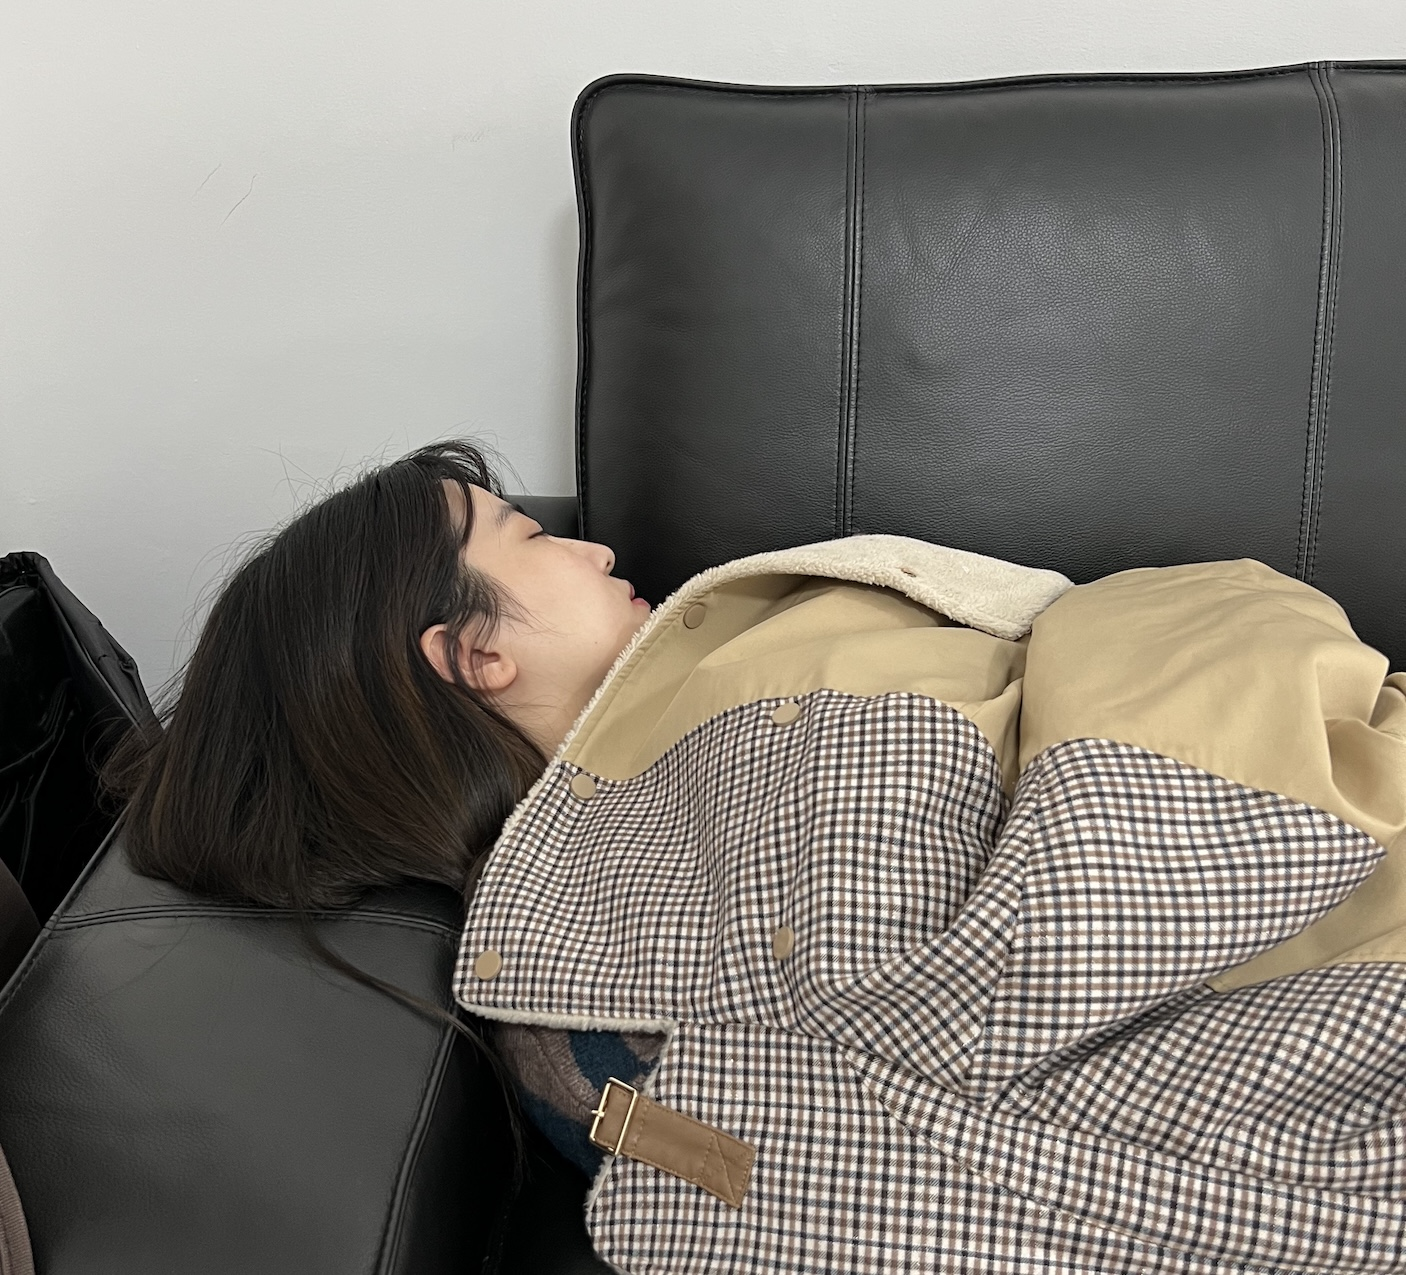
\includegraphics[width=0.75\textwidth]{figures/guo_9.jpg}
\caption{郭菊陽在白石洲}
\end{figure}